\documentclass{article}

\usepackage[left=2cm,right=2cm,top=2cm,bottom=2cm]{geometry} 

\usepackage[utf8]{inputenc}   % otra alternativa para los caracteres acentuados y la "ñ"
\usepackage[           spanish % para poder usar el español
                      ,es-tabla % para los captions de las tablas
                       ]{babel}   
\decimalpoint %para usar el punto decimal en vez de coma para los números con decimales

%\usepackage{beton}
%\usepackage[T1]{fontenc}

\usepackage{parskip}
\usepackage{xcolor}

\usepackage{caption}

\usepackage{fancyvrb}

\usepackage{enumerate} % paquete para poder personalizar fácilmente la apariencia de las listas enumerativas

\usepackage{graphicx} % figuras
\usepackage{subfigure} % subfiguras

\usepackage{amsfonts}
\usepackage{amsmath}

\usepackage[formats]{listings}
\lstdefineformat{R}{~=\( \sim \)}
\lstset{basicstyle=\ttfamily,format=R}

\definecolor{gris}{RGB}{220,220,220}
	
\usepackage{float} % para controlar la situación de los entornos flotantes

\restylefloat{figure}
\restylefloat{table} 
\setlength{\parindent}{0mm}


\usepackage[bookmarks=true,
            bookmarksnumbered=false, % true means bookmarks in 
                                     % left window are numbered
            bookmarksopen=false,     % true means only level 1
                                     % are displayed.
            colorlinks=true,
            allcolors=blue,
            urlcolor=blue]{hyperref}
\definecolor{webblue}{rgb}{0, 0, 0.5}  % less intense blue


\title{\Huge SWAP: Asegurar la granja web\vspace{10mm}}

\author{\huge David Cabezas Berrido \vspace{10mm} \\ 
  \huge dxabezas@correo.ugr.es \vspace{10mm}}

\begin{document}
\maketitle
\tableofcontents
\newpage

\section{Instalar un certificado SSL autofirmado para configurar el acceso por HTTPS}

Para habilitar el módulo SSL de Apache2, ejecutamos la siguiente línea.

\begin{Verbatim}[tabsize=4]
sudo a2enmod ssl 
\end{Verbatim}
Habilita el módulo y sus dependencias. Salida:
\begin{Verbatim}[tabsize=4]
Considering dependency setenvif for ssl:
Module setenvif already enabled
Considering dependency mime for ssl:
Module mime already enabled
Considering dependency socache_shmcb for ssl:
Enabling module socache_shmcb.
Enabling module ssl.
See /usr/share/doc/apache2/README.Debian.gz on how to configure SSL and create self-signed certificates.
To activate the new configuration, you need to run:
systemctl restart apache2
\end{Verbatim}
Restauramos el servicio con \verb^sudo systemctl restart apache2^. Ahora creamos una carpeta para los certificados de Apache, y creamos un par de clave y cerficiado. Le ponemos longitud de clave 2048 bits y 365 de validez.

\begin{figure}[H]
	\centering
	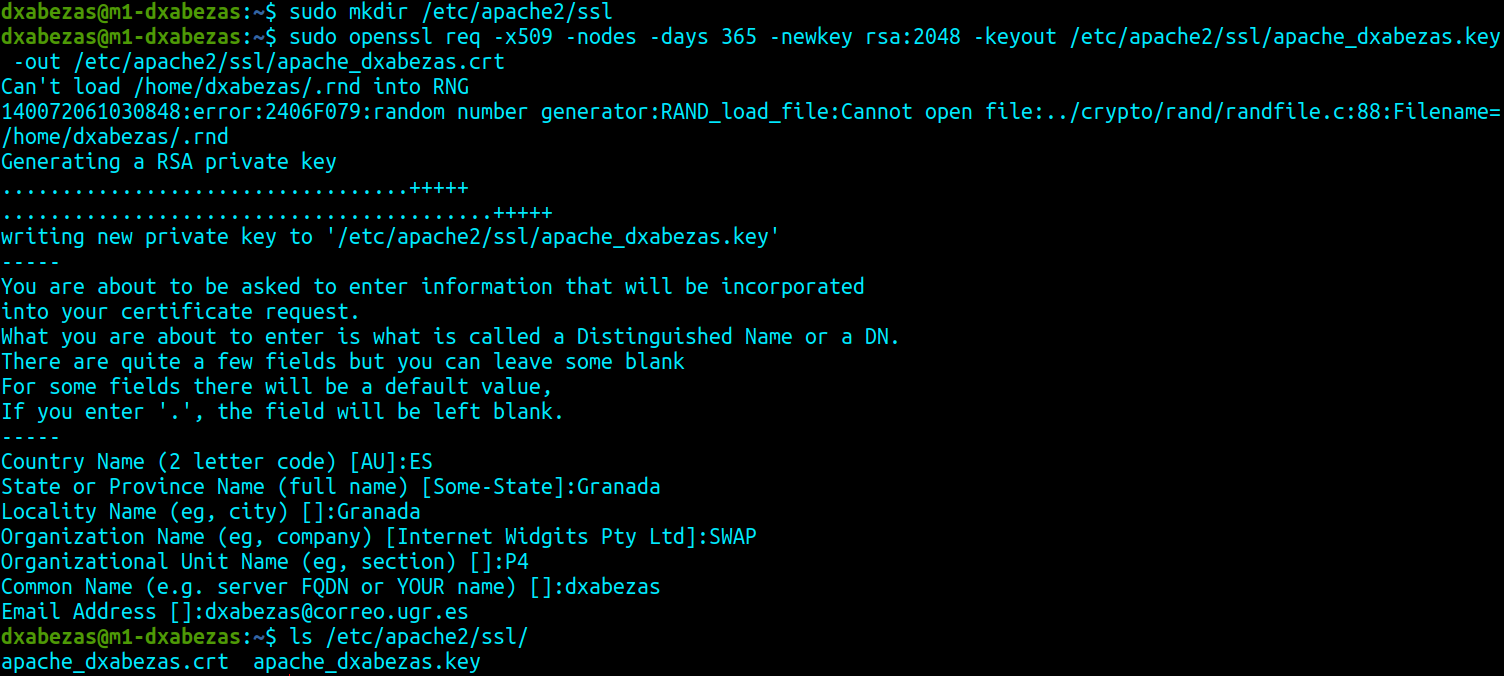
\includegraphics[width=180mm]{imgs/cert-create}
	\caption{Rellenamos los datos del certificado como se indica en el guión. Comprobamos que se ha creado el par correctamente.}
	\label{fig:cert-create}
\end{figure}

Como opciones avanzadas comentamos que \texttt{-x509} auto-firma el certificado, se obtendría una solicitud de certificado si no usásemos
esta opción. Además, la opción \\ \texttt{-subj "/C=TheCountry/CN=theCommonName/ST=theState/O=theOrganization/..."} permite especificar los datos
desde la orden, pueden consultarse las abreviaturas en \href{https://stackoverflow.com/questions/6464129/certificate-subject-x-509}
este post se encuentran los distintos atributos y sus abreviaturas.

Ahora modificamos el fichero de configuración \texttt{/etc/apache2/sites-available/default-ssl.conf}, tenemos que tener el siguiente
bloque (\verb|SSLEngine on| ya estaba puesto).

\begin{Verbatim}[tabsize=4]
#   SSL Engine Switch:
#   Enable/Disable SSL for this virtual host.
SSLEngine on
SSLCertificateFile /etc/apache2/ssl/apache_dxabezas.crt
SSLCertificateKeyFile /etc/apache2/ssl/apache_dxabezas.key
\end{Verbatim}
También tenemos que comentar las líneas que sobreescriben estas directivas más abajo. Guardamos los cambios y ejecutamos
\begin{Verbatim}[tabsize=4]
a2ensite default-ssl
service apache2 reload
\end{Verbatim}

Cuando accedemos a la página, nos avisa de que es insegura porque el certificado es auto-firmado. Debemos permitir la excepción en
el navegador o añadir \texttt{-k} con \texttt{curl}. Si le damos al candado junto a la dirección y a \texttt{More Information},
podemos visualizar el certificado que hemos creado.

\begin{figure}[H]
	\centering
	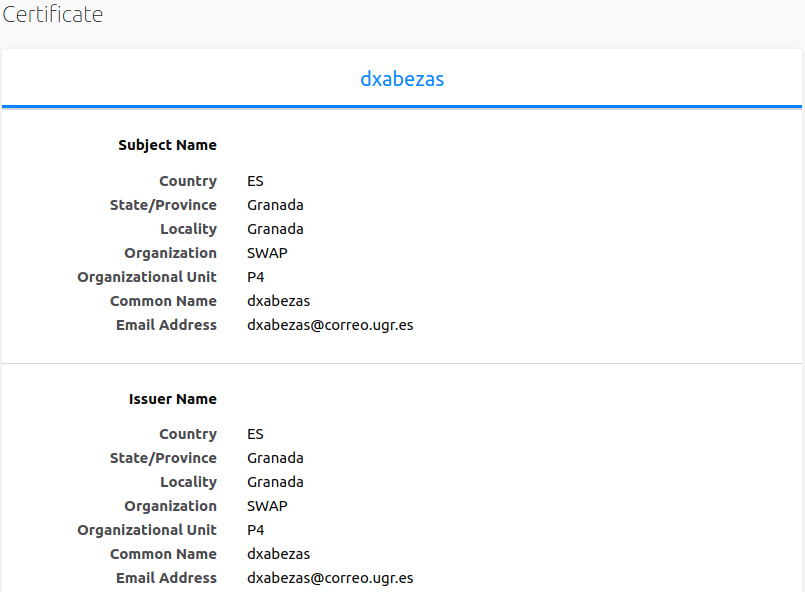
\includegraphics[width=140mm]{imgs/cert-view}
	\caption{Certificado con los datos que hemos creado.}
	\label{fig:cert-view}
\end{figure}

Como opciones avanzadas, mostramos como obtener el certificado sin ayuda del navegador, con \texttt{openssl}:
\begin{Verbatim}[tabsize=4]
openssl s_client -connect 192.168.56.101:443 -showcerts
\end{Verbatim}

También hay varias opciones adicionales en la configuración de Apache2 SSL. Se activan con
\begin{Verbatim}[tabsize=4]
SSLOptions +opcion1 +opcion2
\end{Verbatim}

Por ejemplo, cuando se trabaja con autenticación y se requiere que los clientes también tengan certificados, la opción
\texttt{FakeBasicAuth} requiere que los clientes pongan el campo Subject the su certificado como usuario, la contraseña siempre
es la misma: ``xxj31ZMTZzkVA'' (que es una encriptación por DES de la palabra ``password''), por ello el nombre de Fake.

\section{Configurar la granja web para que permita HTTPS}



\end{document}
